\documentclass[11pt, oneside]{article}  
\usepackage{amsmath, amssymb}
\usepackage[margin=0.5in]{geometry}
\usepackage[ampersand]{easylist}
\usepackage{subcaption}
\usepackage{csquotes}
\usepackage{pgfplots}
\usepackage{tikz}
\usetikzlibrary{arrows.meta}
\pgfplotsset{width=10cm,compat=1.9}


\title{Coursera-Stanford-ML-Notes}
\author{Quentin Truong}
\date{20 June 2017 - ? July 2017}


\begin{document}
\maketitle
\tableofcontents
\pagenumbering{arabic}
\newpage



%======================================================
%========================WEEK 1========================
%======================================================
\section{Week 1: Introduction}
\subsection{Overview}
	\begin{easylist}  
	\ListProperties(Hide=100, Hang=true, Progressive=4ex, Style*=--\ , Style2*=$\bullet\ $)
		& Machine Learning: \hyphenquote{}{A computer program is said to learn from experience E with respect to some class of tasks T and performance measure P, if its performance at tasks in T, as measured by P, improves with experience E.}
		& Supervised Learning: know what our correct output looks like
		&& Regression: want continuous output
		&& Classification: want discrete output
		& Unsupervised Learning: little or no idea what our results should look like
		&& Clustering: find groups according to similarity in various variables 
		&& Nonclustering: find structure in chaos
	\end{easylist}

\newpage



%======================================================
%========================WEEK 2========================
%======================================================
\section{Week 2: Linear Regression with Multiple Variables}
\subsection{Overview}
	\begin{easylist} 
	\ListProperties(Hide=100, Hang=true, Progressive=4ex, Style*=--\ , Style2*=$\bullet\ $)
		& Use linear regression for continuous output
		& Choose gradient descent if many features (million+) because the inverse matrix required for the normal equation can become expensive to compute
		& Normal equation will directly compute theta
		& Normalize features if using gradient descent
	\end{easylist}

\subsection{Symbols}
	\begin{align*}
		m &= number\ of\ samples\\
		n &= number\ of\ feature\\
		x &= (n \times 1)\\
		X &= (m \times n)\\
		X_j &= (m \times 1)\\
		\theta &= (n \times 1)\\
		\theta_j &= (1 \times 1)
	\end{align*}

\subsection{Gradient Descent}
	\begin{align*}
		\text{Hypothesis Function} && 
			h_\theta(x) &= \theta^\intercal \times x\\
		\text{Vectorized Hypothesis Function} && 
			h_\theta(X) &= X \cdot \theta \\
		\text{Linear Regression Cost Function} && 
			J(\theta) &= \frac{1}{2 m} \sum (h_\theta(X) - y)^2 \\
		\text{Derivative of Linear Regression CF wrt $\theta_j$} && 
			\frac{\partial}{\partial \theta_j} J(\theta) &= \frac{1}{m} \sum (h_\theta(X) - y)\ .* X_j \\
		\text{Change in $\theta_j$} &&
			\theta_j &= \theta_j - \alpha \frac{\partial}{\partial \theta_j} \\
		\text{} &&
			&= \theta_j - \alpha \frac{1}{m} \sum (h_\theta(X) - y)\ .* X_j \\
		\text{Vectorized Change in $\theta$} &&
			\theta &= \theta - \alpha \frac{1}{m} X^\intercal (X \cdot \theta - y) 
	\end{align*}

\subsection{Normal Equation}
	\begin{align*}
		\theta &= (X^\intercal \cdot X)^\text{-1} \cdot X^\intercal \cdot y
	\end{align*}

\newpage



%======================================================
%========================WEEK 3========================
%======================================================
\section{Week 3: Logistic Regression}
\subsection{Overview}
	\begin{easylist} 
	\ListProperties(Hide=100, Hang=true, Progressive=4ex, Style*=--\ , Style2*=$\bullet\ $)
		& Use logistic regression for discrete output (classification)
		&& $h_\theta(x)=(y=1|x;\theta)$; gives probability that the output is 1 given $x$
		&& Sigmoid/Logistic function maps any real number to (0, 1)
		&& For multi-class classification, use one-vs-all
		&& Pick class i that maximizes $h^i_\theta(x)$
		& Overfitting is when learned hypothesis fits training data well but fails to generalize
		&& Underfitting is when doesn't fit training data
		& Address overfitting by reducing number of features, model selection, and regularization
		&& Regularization results in simpler hypothesis and less overfitting
		&& Extremely large $\lambda$ will result in underfitting and gradient descent will fail to converge
		&& Do not regularize $\lambda_0$
		& Use other prewritten optimization algorithims (conjugate gradient, BFGS, L-BFGS) because they are faster
	\end{easylist}

\subsection{Logistic Regression Hypothesis Function}
	\begin{align*}
		\text{Sigmoid/Logistic\ Function} && 
			g(z) &= \frac{1}{1+e^{-z}} \\
		\text{Hypothesis\ Function} && 
			h_\theta(x) &= g(\theta^\intercal x) \\
		\text{} && 
			&= \frac{1}{1+e^{-\theta^\intercal x}} 
	\end{align*}

\subsection{Logistic Regression Cost Function}
	\begin{align*}
		Cost(h_\theta(x), y) &= 
			\begin{cases} 
				-\log(h_\theta(x)) \text{ if y = 1 } \\
				-\log(1 - h_\theta(x)) \text{ if y = 0}
			\end{cases}\\
		&= -y\log(h_\theta(x)) - (1-y)\log(1 - h_\theta(x)) \\
		J(\theta) &= \frac{1}{m} \sum^m_{i=1}\text{Cost}(h_\theta(x^i),y^i) \\
		J(\theta) &= \frac{-1}{m} \sum^m_{i=1} \left[y^i\log(h_\theta(x^i)) + (1-y^i)\log(1 - h_\theta(x^i))\right] 
	\end{align*}
\iffalse
	\begin{figure}[!h]
		\begin{subfigure}{.5\textwidth}
			\centering
			\begin{tikzpicture}[scale=0.6]
				\begin{axis}[
					axis lines = left,
					xmin=0, xmax=1, ymin=0, ymax=1,
					xlabel = $h_\theta(x)$,
					ylabel = {$f(x)$},
				]
				\addplot [
					domain=0:1,
					samples=100, 
					color=red,
				]
				{-ln(x)/ln(10)};
				\end{axis}
			\end{tikzpicture}
			\caption{if y=1}
			\label{fig:sub1}
		\end{subfigure}%
		\begin{subfigure}{.5\textwidth}
			\centering
			\begin{tikzpicture}[scale=0.6]
				\begin{axis}[
					axis lines = left,
					xmin=0, xmax=1, ymin=0, ymax=1,
					xlabel = $h_\theta(x)$,
					ylabel = {$f(x)$},
				]
				\addplot [
					domain=0:1,
					samples=100, 
					color=red,
				]
				{-ln(1-x)/ln(10)};
				\end{axis}
			\end{tikzpicture}
			\caption{if y=0}
			\label{fig:sub2}
		\end{subfigure}
	\end{figure}
\fi

\subsection{Proof of Logistic Regression Cost Function Derivative}
	\begin{align*}
		J(\theta) &= \frac{-1}{m} \sum^m_{i=1} [y^i\log(h_\theta(x^i)) + (1-y^i)\log(1 - h_\theta(x^i))] \\
		\log(h_\theta(x^i)) &= \log(\frac{1}{1+e^{-\theta x^i}}) = -\log(1+e^{-\theta x^i})\\
		\log(1 - h_\theta(x^i)) &= \log(1-\frac{1}{1+e^{-\theta x^i}})=\log(e^{-\theta x^i})-\log(1+e^{-\theta x^i})=-\theta x^i-\log(1+e^{-\theta x^i})\\
		J(\theta) &= -\frac{1}{m}\sum_{i=1}^m \left[-y^i(\log(1+e^{-\theta x^i})) + (1-y^i)(-\theta x^i-\log(1+e^{-\theta x^i}))\right]\\
		&= -\frac{1}{m}\sum_{i=1}^m \left[y^i\theta x^i - \theta x^i - \log(1+e^{-\theta x^i})\right]\\
		&= -\frac{1}{m}\sum_{i=1}^m \left[y^i\theta x^i -\log(e^{\theta x^i}) - \log(1 + e^{-\theta x^i})\right]\\
		&=-\frac{1}{m}\sum_{i=1}^m \left[y^i\theta x^i - \log(1+e^{\theta x^i})\right]\\
		\frac{\partial}{\partial \theta_j}y^i\theta x^i &= y^i x^i_j\\
		\frac{\partial}{\partial \theta_j}\log(1+e^{\theta x^i}) &= \frac{x^i_je^{\theta x^i}}{1+e^{\theta x^i}}\\
		&= \frac{{x^i_j}}{{1+e^{-\theta x^i}}}\\
		&= x^i_jh_\theta(x^i)\\
		\frac{\partial}{\partial \theta_j}J(\theta) &= -\frac{1}{m}\sum_{i=1}^m \left[y^i x^i_j - x^i_jh_\theta(x^i)\right]\\
		\frac{\partial}{\partial \theta_j}J(\theta) &= \frac{1}{m}\sum_{i=1}^m \left[h_\theta(x^i) - y^i\right]x^i_j
	\end{align*}

\subsection{Regularization}
	\begin{align*}
		\text{Regularizing Term} &&
			& \lambda \sum_{j=1}^n \theta_j^2\\
		\text{Regularized Linear Regression CF} &&
			J(\theta) &= \frac{1}{2 m} \sum_{i=1}^m (h_\theta(x^i) - y^i)^2 + \lambda \sum_{j=1}^n \theta_j^2\\
		\text{Regularized Logistic Regression CF} &&
			J(\theta) &= \frac{-1}{m} \sum^m_{i=1} \left[y^i\log(h_\theta(x^i)) + (1-y^i)\log(1 - h_\theta(x^i))\right] + \frac{\lambda}{2m} \sum_{j=1}^n \theta_j^2\\
		\text{Regularized GD (Lin/Log Regression)} &&
			& \begin{cases} 
				\theta_0 = \theta_j - \alpha \left[\frac{1}{m}\sum_{i=1}^m (h_\theta(x^i) - y^i)x_0^i\right]\\
				\theta_j = \theta_j - \alpha \left[\frac{1}{m}\sum_{i=1}^m (h_\theta(x^i) - y^i)x_j^i + \frac{\lambda}{m}\theta_j\right] \text{(j=1,2,...,n)}
			\end{cases}\\
		\text{Regularized Normal Equation} &&
			\theta &= (X^\intercal X + \lambda 
			\begin{bmatrix} 
				0 & 0 & \cdots & 0 \\
  				0 & 1 & \cdots & 0 \\
				\vdots  & \vdots  & \ddots & \vdots  \\
				0 & 0 & \cdots & 1 
			\end{bmatrix}_{n+1,n+1}
			)^{-1} X^\intercal y
	\end{align*}

\newpage



%======================================================
%========================WEEK 4========================
%======================================================
\section{Week 4: Artificial Neural Networks Representation}
\subsection{Overview}
	\begin{easylist} 
	\ListProperties(Hide=100, Hang=true, Progressive=4ex, Style*=--\ , Style2*=$\bullet\ $)
		& Neural networks allow for non-linear classification in situations with many features
		&& Necessary b/c 100 features at 3rd level polynomials generates 170k features, which quickly becomes intractable
		&& \hyphenquote{}{One learning algorithm} hypothesis; you can see with your tongue : brain learns using one algorithm, not thousands of different programs
		& General
		&& If network has $s_j$ units in layer $j$ and $s_{j+1}$ units in layer $j+1$, then $\Theta^j$ will be of dimension $s_{j+1} \times s_j+1$
		&&& The +1 comes from the addition in $\Theta^{(j)}$ of the bias node, $x_0$ and $\Theta_0^{(j)}$
		&& Can have multiple hidden layers
		&& Can have multiple outputs (one-vs-all for multi-class classification)
		&& If three layers:
		&&& Layer 1: Input nodes
		&&& Layer 2: Hidden/intermediate layer
		&&& Layer 3: Output layer
		& Forward Propogation is used to predict based on learned parameters
		& Bias node gives each node a trainable constant value
		&& Allows bias weight to shift the activation curve left/right
		&& Other weights affect steepness
	\end{easylist}

\subsection{Symbols}
	\begin{easylist} 
	\ListProperties(Hide=100, Hang=true, Progressive=4ex, Style*=--\ , Style2*=$\bullet\ $)
		& $g(x)$: sigmoid function
		& $a_i^{(j)}$: \hyphenquote{}{activation} of unit i in layer j
		& $\Theta^{(j)}$: matrix of weights controlling function mapping from layer j to layer j+1; each layer gets own $\Theta^j$
		& $z_k^{(j)}$: encompasses parameters inside of g function (from above)
	\end{easylist}

\subsection{Equations}
	\begin{align*}
		z_k^{(j)} &= \Theta_{k,0}^{(j-1)}x_0 + \Theta_{k,1}^{(j-1)}x_1 + ... + \Theta_{k,n}^{(j-1)}x_n \\
		&= \Theta_{k,0}^{(j-1)}a_0^{(j-1)} + \Theta_{k,1}^{(j-1)}a_1^{(j-1)} + ... + \Theta_{k,n}^{(j-1)}a_n^{(j-1)} \\
		z^{(j)} &= \Theta^{(j-1)}a^{(j-1)} \\
		a^{(j)} &= g(z^{(j)})
	\end{align*}

\subsection{Sample Three Layer System}
\begin{figure}[!h]
    \centering
    \begin{minipage}{.5\textwidth}
    	\centering
        \begin{equation*}
			\begin{bmatrix} 
				x_0 \\
				x_1 \\
				x_2 \\
				x_3 \\
			\end{bmatrix}
			\rightarrow
			\begin{bmatrix} 
				a_1^{(2)} \\
				a_2^{(2)} \\
				a_3^{(2)} \\
			\end{bmatrix}
			\rightarrow
			h_\Theta(x)
		\end{equation*}
		\begin{align*}
			a_1^{(2)} &= g(\Theta_{1,0}^{(1)} x_0 + \Theta_{1,1}^{(1)} x_1 + \Theta_{1,2}^{(1)} x_2 + \Theta_{1,3}^{(1)} x_3) \\
			a_2^{(2)} &= g(\Theta_{2,0}^{(1)} x_0 + \Theta_{2,1}^{(1)} x_1 + \Theta_{2,2}^{(1)} x_2 + \Theta_{2,3}^{(1)} x_3) \\
			a_3^{(2)} &= g(\Theta_{3,0}^{(1)} x_0 + \Theta_{3,1}^{(1)} x_1 + \Theta_{3,2}^{(1)} x_2 + \Theta_{3,3}^{(1)} x_3) \\
			h_\Theta(x) &= g(\Theta_{1,0}^{(2)} a_0^{(2)} + \Theta_{1,1}^{(2)} a_1^{(2)} + \Theta_{1,2}^{(2)} a_2^{(2)} + \Theta_{1,3}^{(2)} a_3^{(2)})\\
			&= g(z^3)\\
			&= a_1^{(3)}
		\end{align*}
    \end{minipage}%
    \begin{minipage}{0.5\textwidth}
    	\centering
    	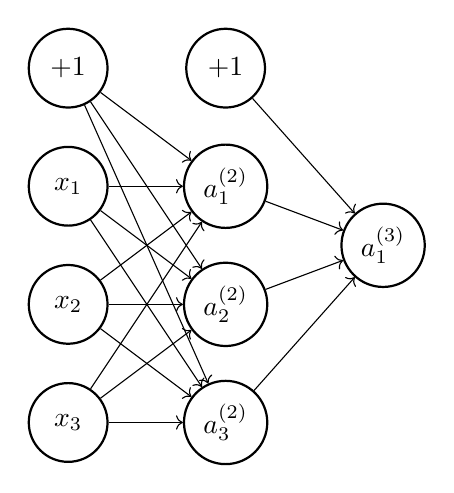
\begin{tikzpicture}
			\begin{scope}[every node/.style={circle,thick,draw,minimum size=10mm}]
				\node (x_0) at (0,4.5) {$+1$};
				\node (x_1) at (0,3) {$x_1$};
				\node (x_2) at (0,1.5) {$x_2$};
				\node (x_3) at (0,0) {$x_3$};

				\node (a_0^2) at (2,4.5) {$+1$};
				\node (a_1^2) at (2,3) {$a_1^{(2)}$};
				\node (a_2^2) at (2,1.5) {$a_2^{(2)}$};
				\node (a_3^2) at (2,0) {$a_3^{(2)}$};

				\node (a_1^3) at (4,2.25) {$a_1^{(3)}$};
			\end{scope}
			\begin{scope}[]
				\path [->] (x_0) edge node {} (a_1^2);
				\path [->] (x_0) edge node {} (a_2^2);
				\path [->] (x_0) edge node {} (a_3^2);

				\path [->] (x_1) edge node {} (a_1^2);
				\path [->] (x_1) edge node {} (a_2^2);
				\path [->] (x_1) edge node {} (a_3^2);

				\path [->] (x_2) edge node {} (a_1^2);
				\path [->] (x_2) edge node {} (a_2^2);
				\path [->] (x_2) edge node {} (a_3^2);

				\path [->] (x_3) edge node {} (a_1^2);
				\path [->] (x_3) edge node {} (a_2^2);
				\path [->] (x_3) edge node {} (a_3^2);

				\path [->] (a_0^2) edge node {} (a_1^3);
				\path [->] (a_1^2) edge node {} (a_1^3);
				\path [->] (a_2^2) edge node {} (a_1^3);
				\path [->] (a_3^2) edge node {} (a_1^3);
			\end{scope}
		\end{tikzpicture}
    \end{minipage}
\end{figure}

\newpage



%======================================================
%========================WEEK 5========================
%======================================================
\section{Week 5: Artificial Neural Network Learning}
\subsection{Symbols}
	\begin{easylist} 
	\ListProperties(Hide=100, Hang=true, Progressive=4ex, Style*=--\ , Style2*=$\bullet\ $)
		& $L$ : total number of layers in the network
		& $s_l$ : number of units (not counting bias unit) in layer $l$
		& $K$ : number of output units/classes
		& $h_\Theta(x)_k$ : hypothesis that results in the kth output
	\end{easylist}

\subsection{Cost Function}
	\begin{equation*}
		J(\Theta) = - \frac{1}{m} \sum_{i=1}^m \sum_{k=1}^K \left[y^{(i)}_k \log ((h_\Theta (x^{(i)}))_k) + (1 - y^{(i)}_k)\log (1 - (h_\Theta(x^{(i)}))_k)\right] + \frac{\lambda}{2m}\sum_{l=1}^{L-1} \sum_{i=1}^{s_l} \sum_{j=1}^{s_{l+1}} ( \Theta_{j,i}^{(l)})^2
	\end{equation*}
	\begin{align*}
		\text{Picks training example} && 
			\sum_{i=1}^m\\
		\text{Picks output node} && 
			\sum_{k=1}^K\\
		\text{Picks layer} && 
			\sum_{l=1}^{L-1}\\
		\text{Picks node} && 
			\sum_{i=1}^{s_l}\\
		\text{Picks $\Theta$} && 
			\sum_{j=1}^{s_{l+1}}\\
	\end{align*}

\subsection{Backpropagation Algorithm}
\begin{enumerate}
	\item Set $a(1):=x(t)$
	\item Perform forward propagation to compute $a(l)$ for $l=2,3,…,L$
	\item Using $y^{(t)}$, compute $\delta^L=a^{(L)} - y^{(t)}$
	\item Compute $\delta^{(L-1)}, \delta^{(L-2)},\dots,\delta^{(2)}$ using $\delta^{(l)} = ((\Theta^{(l)})^T \delta^{(l+1)})\ .*\ a^{(l)}\ .*\ (1 - a^{(l)})$
	\item $\Delta^{(l)}_{i,j} := \Delta^{(l)}_{i,j} + a_j^{(l)} \delta_i^{(l+1)}$ or with vectorization $\Delta^{(l)} := \Delta^{(l)} + \delta^{(l+1)}(a^{(l)})^\intercal$
	\item $\frac \partial {\partial \Theta_{ij}^{(l)}} J(\Theta) = D_{ij}^{(l)}$ where 
		$\begin{cases}
			D^{(l)}_{i,j} := \dfrac{1}{m}\Delta^{(l)}_{i,j} \text{ (j = 0)}\\
			D^{(l)}_{i,j} := \dfrac{1}{m}\left(\Delta^{(l)}_{i,j} + \lambda\Theta^{(l)}_{i,j}\right) \text{ (j $\neq$ 0)}
		\end{cases}$
\end{enumerate}

\subsection{Backpropagation Error Derivation}
	\begin{align*}
		\delta_j^{(l)} &= \dfrac{\partial}{\partial z_j^{(l)}} cost(t)\\
		\delta^{(l)} &= ((\Theta^{(l)})^T \delta^{(l+1)})\ .* g^\prime(z^{(l)}) \\
		g^\prime(z^{(l)}) &= a^{(l)}\ .*\ (1 - a^{(l)})
	\end{align*}

\subsection{Gradient Checking}
\begin{easylist} 
	\ListProperties(Hide=100, Hang=true, Progressive=4ex, Style*=--\ , Style2*=$\bullet\ $)
		& Gradient checking ensures that backpropagation is actually working
		&& Turn off gradient checking once backpropagation is verified to work
		& Approximate the derivative of cost function using slope
		&& Pick $\epsilon = 10^{-4}$
		&& Check all $\Theta_j$
	\end{easylist}
	\begin{equation*}
		\dfrac{\partial}{\partial\Theta_j}J(\Theta) \approx \dfrac{J(\Theta_1, \dots, \Theta_j + \epsilon, \dots, \Theta_n) - J(\Theta_1, \dots, \Theta_j - \epsilon, \dots, \Theta_n)}{2\epsilon}
	\end{equation*}

\subsection{Random Initialization}
	\begin{easylist} 
	\ListProperties(Hide=100, Hang=true, Progressive=4ex, Style*=--\ , Style2*=$\bullet\ $)
		& Need Symmetry Breaking
		&& All hidden units would receive the same signal and the same updates
		&& Results in finding only one feature, redundantly copied many times over
		& Fixed by randomly initializing each $\Theta_{ij}^{(l)}$ to a value in $[-\epsilon, \epsilon]$
	\end{easylist}

\newpage










\end{document}  